\documentclass{skyalert-report}

%% ══════════════════════════════════════════════════════════════════════════
%%  DATOS DE LA INSTALACIÓN — Acapulco Palmeiras
%% ══════════════════════════════════════════════════════════════════════════

\sitename{Condominio Residencial Palmeiras A.C.}
\sitelocation{Acapulco, Guerrero}
\siteaddress{Costera de las Palmas 1-Lote H-8A, Playa Diamante, 39890 Acapulco de Ju\'arez, Gro.}
\sitemaps{https://maps.app.goo.gl/KRtSaumbGkwJFvZR6}
\sitelat{16.768045\textdegree{} N}
\sitelong{-99.785777\textdegree{} W}
\sitealt{0 m}
\seismiczone{Tipo D -- Alta Sismicidad}

\stationid{AISensor001}
\sensormodel{AS-Explorer}
\installdate{27 de Marzo de 2026}
\folio{Ruta-Guerero-01-2026}
\reportid{2026-Gro-001}

\authorname{Isaac P\'erez}
\supportnames{Jorge Giles \& Omar Barrag\'an}
\coverlogo{palmeiras_img1}

\newcommand{\contactoA}{Luis Zurita Aca\newline{\small Encargado residencial -- +52 1 744 587 9358}}
\newcommand{\contactoB}{Ing. Cristian Diaz\newline{\small Jefe de mantenimiento -- +52 1 744 533 2469}}

%% ══════════════════════════════════════════════════════════════════════════
\begin{document}

%% ===== PÁG 1: PORTADA =====================================================
\makecover

%% ===== PÁG 2: DATOS GENERALES =============================================
\setheadertext{Datos Generales}
\setfootertext{AISensor001 \textperiodcentered{} Acapulco, Gro. \textperiodcentered{} 27-Mar-2026}

\sectionhead{Datos Generales de la Instalaci\'on}

\begin{card}
\begin{tabular}{@{}p{0.46\textwidth}p{0.46\textwidth}@{}}
\datafield{Nombre del Sitio}{Condominio Residencial Palmeiras A.C.}&
\datafield{Fecha de Instalaci\'on}{27 de Marzo de 2026}\\
\datafield{Folio / ID de Reporte}{2026-Gro-001}&
\datafield{Zona S\'ismica}{Tipo D -- Alta Sismicidad}\\
\end{tabular}%

\begin{tabular}{@{}p{0.95\textwidth}@{}}
\datafield{Direcci\'on}{Costera de las Palmas 1-Lote H-8A, Playa Diamante, 39890 Acapulco de Ju\'arez, Gro.}\\
\datafield{Google Maps}{\small\url{https://maps.app.goo.gl/KRtSaumbGkwJFvZR6}}\\
\end{tabular}%

\begin{tabular}{@{}p{0.30\textwidth}p{0.30\textwidth}p{0.30\textwidth}@{}}
\datafield{Latitud}{16.768045\textdegree{} N}&
\datafield{Longitud}{-99.785777\textdegree{} W}&
\datafield{Altitud}{0 m}\\
\end{tabular}%

\begin{tabular}{@{}p{0.46\textwidth}p{0.46\textwidth}@{}}
\datafield{Contacto en Sitio (1)}{\contactoA}&
\datafield{Contacto en Sitio (2)}{\contactoB}\\
\end{tabular}%
\end{card}

\sectionhead{Detalles de la Estaci\'on S\'ismica}

\begin{tcolorbox}[
  enhanced,colback=tablebg,colframe=divider,boxrule=0.4pt,
  arc=4pt,left=0pt,right=0pt,top=0pt,bottom=0pt,
  shadow={0.4mm}{-0.4mm}{0mm}{black!8}
]
{\footnotesize\setlength{\tabcolsep}{3pt}\raggedright
\begin{tabular}{@{\hspace{4pt}}
  >{\bfseries\raggedright\arraybackslash}p{0.20\textwidth}
  >{\raggedright\arraybackslash}p{0.15\textwidth}
  >{\raggedright\arraybackslash}p{0.08\textwidth}
  >{\raggedright\arraybackslash}p{0.17\textwidth}
  >{\raggedright\arraybackslash}p{0.11\textwidth}
  >{\raggedright\arraybackslash}p{0.12\textwidth}@{\hspace{4pt}}}
\rowcolor{darkbg}
\thead{Dispositivo}&
\thead{Modelo}&
\thead{ID/SN}&
\thead{Ubicaci\'on}&
\thead{Propiedad}&
\thead{Estado}\\
\rowcolor{white}
GPU NVIDIA & Jetson Orin Nano & 01 & Subestaci\'on el\'ectrica & SkyAlert & \chipok{Activo}\\
\rowcolor{tablerow}
Sensor S\'ismico & ASExplorer E-C111G & 04881401 & Subestaci\'on el\'ectrica & SkyAlert & \chipok{Activo}\\
\rowcolor{white}
Sensor S\'ism. Sec. & SKYACC & -- & Subestaci\'on el\'ectrica & SkyAlert & \chipok{Activo}\\
\rowcolor{tablerow}
M\'odem / Router & ZTE / Telcel & -- & Subestaci\'on el\'ectrica & SkyAlert & \chipok{Activo}\\
\rowcolor{white}
Antena Alta Ganancia & Receptora exterior & -- & Subestaci\'on el\'ectrica & SkyAlert & \chipok{Activo}\\
\rowcolor{tablerow}
Regulador de Voltaje & Volteck & -- & Subestaci\'on el\'ectrica & SkyAlert & \chipok{Activo}\\
\rowcolor{white}
Bocina / Altavoz & Ninguna & -- & N/A & -- & \chipna{N/A}\\
\rowcolor{tablerow}
UPS / Bater\'ia & Ninguna & -- & N/A & -- & \chipna{N/A}\\
\end{tabular}}
\end{tcolorbox}

\vspace{5mm}
\noindent
\begin{minipage}[t]{0.24\textwidth}\kpiblock{\faIcon{microchip}}{6}{Dispositivos Activos}\end{minipage}\hfill
\begin{minipage}[t]{0.24\textwidth}\kpiblock{\faIcon{wifi}}{4G}{Conectividad}\end{minipage}\hfill
\begin{minipage}[t]{0.24\textwidth}\kpiblock{\faIcon{shield-alt}}{24 bit}{Resoluci\'on ADC}\end{minipage}\hfill
\begin{minipage}[t]{0.24\textwidth}\kpiblock{\faIcon{clock}}{< 0.1s}{Latencia}\end{minipage}

\newpage

%% ===== PÁG 3: EVIDENCIA FOTOGRÁFICA =======================================
\setheadertext{Evidencia Fotogr\'afica}

\sectionhead{Evidencia Fotogr\'afica de la Instalaci\'on}

\subsectionlabel{Ubicaci\'on del Sitio}

\noindent
\begin{minipage}[t]{0.32\textwidth}
\photoframe{palmeiras_img2}{Condominio Residencial Palmeiras}
\end{minipage}\hfill
\begin{minipage}[t]{0.32\textwidth}
\photoframe{palmeiras_img3}{Recepci\'on trasera de condominio}
\end{minipage}\hfill
\begin{minipage}[t]{0.32\textwidth}
\photoframe{palmeiras_img4}{Cuarto -- Subestaci\'on el\'ectrica}
\end{minipage}

\vspace{4mm}
\subsectionlabel{Instalaci\'on de la Estaci\'on}

\noindent
\begin{minipage}[t]{0.32\textwidth}
\photoframe{palmeiras_img5}{Entorno de la instalaci\'on}
\end{minipage}\hfill
\begin{minipage}[t]{0.32\textwidth}
\photoframe{palmeiras_img6}{Acercamiento}
\end{minipage}\hfill
\begin{minipage}[t]{0.32\textwidth}
\photoframe{palmeiras_img7}{SKYACC instalado}
\end{minipage}

\vspace{4mm}\noindent
\begin{minipage}[t]{0.32\textwidth}
\photoframe{palmeiras_img8}{Momento de la instalaci\'on}
\end{minipage}\hfill
\begin{minipage}[t]{0.32\textwidth}
\photoframe{palmeiras_img9}{Medici\'on de ruido s\'ismico}
\end{minipage}\hfill
\begin{minipage}[t]{0.32\textwidth}
\photoframe{palmeiras_img10}{Jetson Orin Nano instalada}
\end{minipage}

\vspace{4mm}
\sectionhead{Apoyo en Instalaci\'on}

\begin{card}
\begin{tabular}{@{}p{0.30\textwidth}p{0.30\textwidth}p{0.30\textwidth}@{}}
\datafield{Nombre}{Jorge Giles}&
\datafield{Cargo}{Gerente de Operaciones}&
\datafield{Fecha}{27 / 03 / 2026}\\
\datafield{Nombre}{Omar Barrag\'an}&
\datafield{Cargo}{Desarrollador Full Stack}&
\datafield{Fecha}{27 / 03 / 2026}\\
\end{tabular}%
\end{card}

\newpage

%% ===== PÁG 4: VALIDACIÓN DE SEÑAL =========================================
\setheadertext{Validaci\'on de Se\~nal}

\sectionhead{Validaci\'on de Se\~nal S\'ismica en Tiempo Real}

\begin{tcolorbox}[
  enhanced,colback=tablebg,colframe=divider,boxrule=0.4pt,
  arc=4pt,left=0pt,right=0pt,top=0pt,bottom=0pt,
  shadow={0.4mm}{-0.4mm}{0mm}{black!8}
]
{\small\setlength{\tabcolsep}{4pt}
\begin{tabular}{@{\hspace{4pt}}
  >{\bfseries\raggedright\arraybackslash}p{0.42\textwidth}
  >{\raggedright\arraybackslash}p{0.28\textwidth}
  >{\raggedright\arraybackslash}p{0.16\textwidth}@{\hspace{4pt}}}
\rowcolor{darkbg}
\thead{Par\'ametro}&
\thead{Valor}&
\thead{Estado}\\
\rowcolor{white}
Nivel de ruido s\'ismico (RMS)&%
\begin{tikzpicture}[baseline=1.5pt]
  \fill[divider,rounded corners=1pt](0,0)rectangle(2.2cm,5pt);
  \fill[greenaccent,rounded corners=1pt](0,0)rectangle(0.66cm,5pt);
\end{tikzpicture}&\chipok{Aceptable}\\
\rowcolor{tablerow}
Frecuencia de muestreo&100 sps&\chipok{OK}\\
\rowcolor{white}
Latencia de transmisi\'on&< 0.1 s&\chipok{OK}\\
\rowcolor{tablerow}
Uptime de conexi\'on&99.8\%&\chipok{OK}\\
\rowcolor{white}
SNR (Signal-to-Noise Ratio)&--&\chipwarn{Pendiente}\\
\rowcolor{tablerow}
Resoluci\'on del ADC&24 bits&\chipok{OK}\\
\rowcolor{white}
Drift de reloj (GPS sync)&< 1 ms&\chipok{OK}\\
\end{tabular}}
\end{tcolorbox}

\vspace{5mm}
\subsectionlabel{Medici\'on de Ruido S\'ismico en Sitio}

\begin{center}
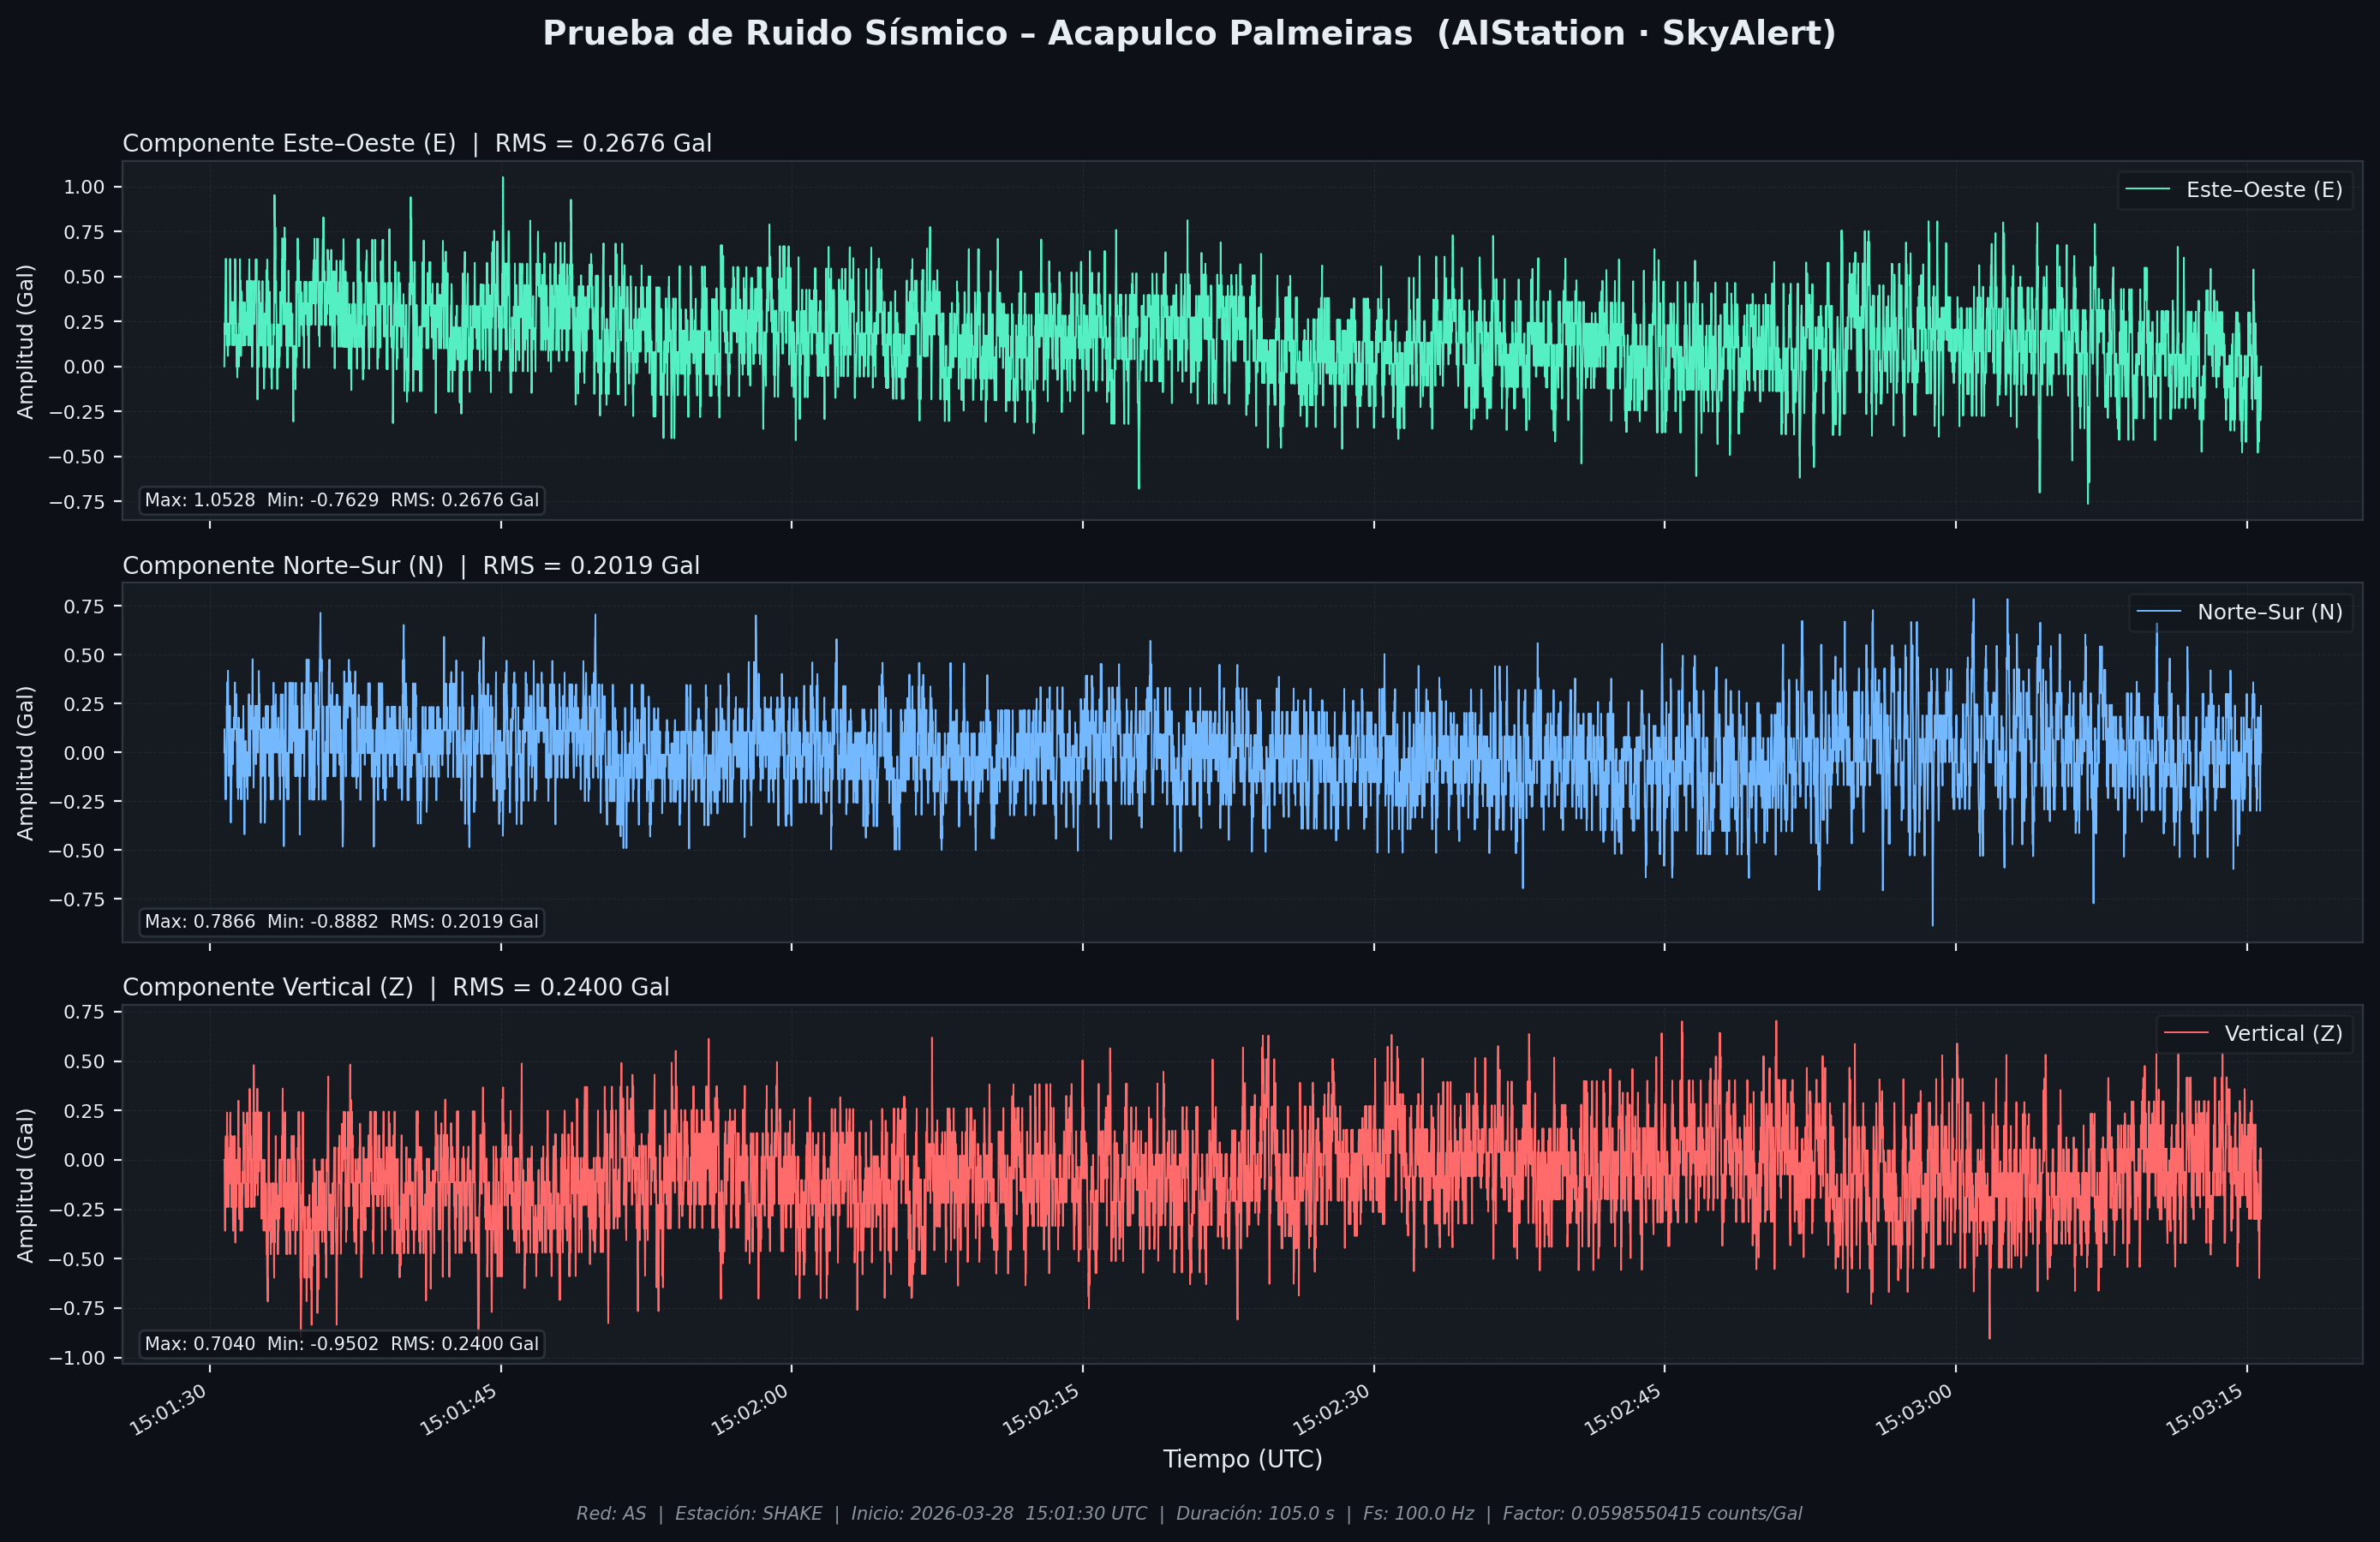
\includegraphics[width=\textwidth]{palmeiras_img11}\\[2mm]
{\small\itshape\textcolor{steel}{Formas de onda de aceleraci\'on registradas durante la medici\'on de ruido s\'ismico en sitio.}}
\end{center}

\newpage

%% ===== PÁG 5: PRUEBA MQTT =================================================
\setheadertext{Prueba MQTT}

\sectionhead{Prueba MQTT -- Mensajes de Anomal\'ia a AWS}

\begin{tcolorbox}[
  enhanced,colback=mqttbg,colframe=mqttframe,boxrule=0.5pt,
  arc=4pt,left=8pt,right=8pt,top=6pt,bottom=6pt,
  shadow={0.5mm}{-0.5mm}{0mm}{black!20}
]
{\ttfamily\small\textcolor{mqttgreen}{\faIcon{terminal}\enspace skyalert-mqtt-client}}%
\hfill
\begin{tikzpicture}[baseline=1pt]
  \node[fill=mqttgreen!20!mqttbg,rounded corners=2pt,inner xsep=4pt,inner ysep=1.5pt]{%
    \bfseries\tiny\textcolor{mqttgreen}{\textbullet{} CONNECTED}%
  };
\end{tikzpicture}\\[3mm]
{\ttfamily\footnotesize
\textcolor{mqttcyan}{broker}\hspace{10mm}\textcolor{mqttdim}{xxxxxxxxxx.iot.us-east-1.amazonaws.com}\\
\textcolor{mqttcyan}{topic}\hspace{11.5mm}\textcolor{mqttdim}{skyalert/earthquake/anomalies}\\
\textcolor{mqttcyan}{mensajes}\hspace{6mm}\textcolor{mqttdim}{4 / 4 (100\%)}\hspace{3mm}\textcolor{mqttgreen}{\faIcon{check-circle}\enspace PASS -- Todos los mensajes entregados}\\[3mm]
\textcolor{mqttframe}{\% PAYLOAD ANOMAL\'IA DETECTADA}\\
\textcolor{mqttdim}{\{}\\
\hspace{4mm}\textcolor{mqttcyan}{"station\_id":}\hspace{2mm}\textcolor{mqttcyan!70!white}{"AISensor001"},\\
\hspace{4mm}\textcolor{mqttcyan}{"message":}\hspace{4mm}\textcolor{mqttcyan!70!white}{"ANOMALIA DETECTADA + IA ACTIVADA}\\
\hspace{4mm}\textcolor{mqttcyan!70!white}{en 2026-03-27 16:45:36 (PGA: 2.5 Gals)"},\\
\hspace{4mm}\textcolor{mqttcyan}{"pga\_gals":}\hspace{3mm}\textcolor{accent}{2.54,}%
\hspace{3mm}\textcolor{mqttcyan}{"anomaly\_active":}\hspace{1mm}\textcolor{amberdark}{true},\\
\hspace{4mm}\textcolor{mqttcyan}{"timestamp":}\hspace{2mm}\textcolor{mqttcyan!70!white}{"2026-03-27T16:45:36.045826+00:00"},\\
\hspace{4mm}\textcolor{mqttcyan}{"location\_name":}\textcolor{mqttcyan!70!white}{"Acapulco, Gro."}\\
\textcolor{mqttdim}{\}}
}
\end{tcolorbox}

\vspace{5mm}
\subsectionlabel{Confirmaci\'on en AWS}

\begin{center}
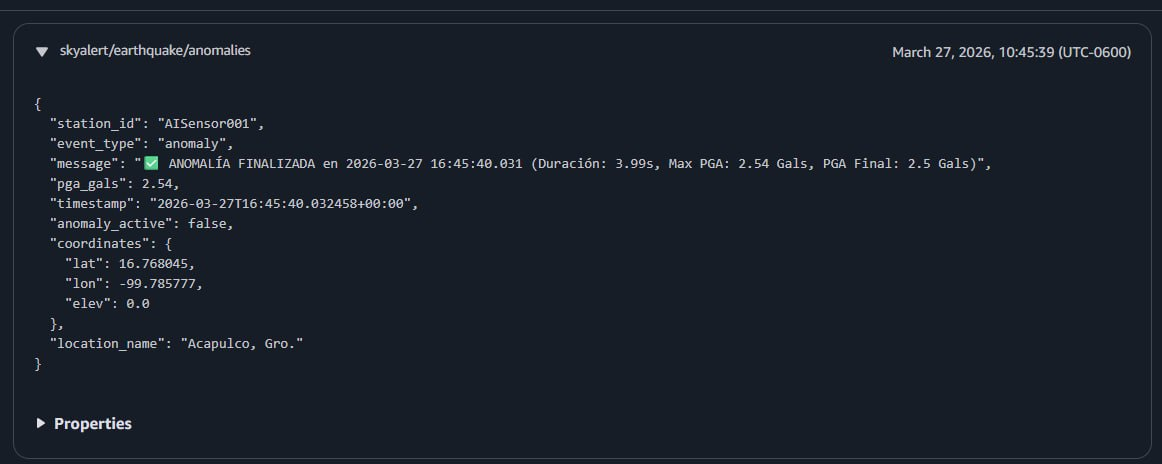
\includegraphics[width=\textwidth]{palmeiras_img12}\\[2mm]
{\small\itshape\textcolor{steel}{Confirmaci\'on de recepci\'on de mensajes de anomal\'ia s\'ismica en los servicios AWS.}}
\end{center}

\newpage

%% ===== PÁG 6: OBSERVACIONES Y FIRMAS ======================================
\setheadertext{Observaciones y Aceptaci\'on}

\sectionhead{Comentarios y Observaciones}

\begin{obsbox}
\justifying
Se realiz\'o un recorrido en el establecimiento para identificar la ubicaci\'on \'optima de la estaci\'on s\'ismica. Debido a que el permiso para la instalaci\'on en pozo a\'un no est\'a autorizado ---ya que se requiere presentar una propuesta est\'etica---, se determin\'o como mejor alternativa el cuarto de la subestaci\'on el\'ectrica, por ser un sitio con m\'inima interferencia vibracional.
\end{obsbox}

\vspace{2mm}
\begin{enumerate}[leftmargin=*,label=\textbf{\textcolor{skyred}{\arabic*.}},itemsep=1pt]
\item Aceler\'ometros anclados al suelo dentro de la subestaci\'on el\'ectrica.
\item Jetson Orin Nano anclada al muro dentro de la subestaci\'on el\'ectrica con clima apropiado para esta.
\item Se instal\'o antena receptora de mayor ganancia para mayor estabilidad de la conexi\'on a internet.
\item La instalaci\'on cumple los est\'andares de calidad SkyAlert 2026.
\end{enumerate}

\vspace{3mm}
\sectionhead{Resumen de Pruebas Realizadas}

\begin{tcolorbox}[
  enhanced,colback=tablebg,colframe=divider,boxrule=0.4pt,
  arc=4pt,left=0pt,right=0pt,top=0pt,bottom=0pt,
  shadow={0.4mm}{-0.4mm}{0mm}{black!8}
]
{\small\setlength{\tabcolsep}{4pt}
\begin{tabular}{@{\hspace{4pt}}
  >{\bfseries\raggedright\arraybackslash}p{0.44\textwidth}
  >{\raggedright\arraybackslash}p{0.14\textwidth}
  >{\raggedright\arraybackslash}p{0.26\textwidth}@{\hspace{4pt}}}
\rowcolor{darkbg}
\thead{Prueba}&
\thead{Resultado}&
\thead{Observaci\'on}\\
\rowcolor{white}
Encendido y arranque del sensor&\chipok{PASS}&Arranque sin errores\\
\rowcolor{tablerow}
Conectividad a internet (Telcel 4G)&\chipok{PASS}&Se\~nal 4G estable\\
\rowcolor{white}
Transmisi\'on de se\~nal s\'ismica&\chipok{PASS}&Latencia < 0.1 s\\
\rowcolor{tablerow}
Medici\'on de ruido s\'ismico del sitio&\chipok{PASS}&< 1.0 cm/s\textsuperscript{2} RMS\\
\rowcolor{white}
Detecci\'on de anomal\'ia (AI Station)&\chipok{PASS}&IA\_output, Zc, PGA\\
\rowcolor{tablerow}
Env\'io MQTT a AWS IoT Core&\chipok{PASS}&4/4 mensajes (100\%)\\
\rowcolor{white}
Sincronizaci\'on de reloj GPS&\chipok{PASS}&Drift < 10 ms\\
\rowcolor{tablerow}
Est\'andares SkyAlert 2026&\chipok{PASS}&Criterios verificados\\
\end{tabular}}
\end{tcolorbox}

\vspace{4mm}
\sectionhead{Verificaci\'on y Aceptaci\'on}

\noindent
\begin{minipage}[t]{0.48\textwidth}
\signblock{Encargado de la Instalaci\'on}{Ing. Isaac P\'erez}{Especialista en Sismolog\'ia e Instrumentaci\'on Geof\'isica}{27 / 03 / 2026}
\end{minipage}\hfill
\begin{minipage}[t]{0.48\textwidth}
\signblock{Encargado del Sitio (Aliado)}{Luis Zurita Aca}{Encargado residencial}{27 / 03 / 2026}
\end{minipage}

\end{document}
